\documentclass[]{article}
\usepackage{algorithm, algpseudocode}
\usepackage{amsmath,amssymb,amsthm,amsfonts}
\usepackage{caption}
\usepackage{comment}
\usepackage{graphicx,verbatim}
\usepackage{listings}
\usepackage{subcaption}

\usepackage[backend=bibtex,style=ieee]{biblatex}
\addbibresource{refs.bib}

\theoremstyle{definition}
\newtheorem{definition}{Definition}[section]

\newcommand{\x}{\mathbf{x}}
\def\bif{\bf if~}
\def\belif{{\bf else if~}}
\def\bthen{{\bf then predict~}}
\def\belse{{\bf else predict~}}

\begin{document}

\title{Accelerating the Search for Certifiably Optimal Rule Lists}
\author{Nicholas Larus-Stone}
\date{3/31/17}
\maketitle

\begin{center}
Abstract
\end{center}

We demonstrate a new algorithm that finds an optimal rule list as well as providing proof of that optimality. Rule lists, which are lists composed of If-Then statements, are similar to decision tree classifiers and are useful because each step in the model's decision making process is understandable by humans. Our algorithm, called CORELS, finds the optimal rule list through the use of three types of bounds: bounds inherent to the rules themselves, bounds based on the current best solution, and bounds based on symmetry between rule lists. We propose novel data structures to minimize the memory usage and runtime of our algorithm on this exponentially difficult problem. One advantage of our algorithm is that it generates not only the optimal rule list and a certificate of optimality, but also the entire solution space of nearly optimal solutions. Our algorithm therefore allows for the analysis and discovery of all optimal and near-optimal solutions on problems requiring human-interpretable algorithms.

\section{Introduction}

As machine learning continues to grow in importance, the interpretability of predictive models remains a crucial problem.
Our goal is to build models that are highly predictive but in which each step of the model's decision making process can also be understood by humans.
Machine learning models such as neural nets or support vector machines are able to achieve stunning predictive accuracy, but the reasons for these predictions remain unintelligible to a human user.
This lack of interpretability is important because models that are not understood by humans can have hidden bias in their predictive decision making.
A recent ProPublica article found racial bias in the use of black box machine learning models used for advising criminal sentencing \cite{LarsonMaKiAn16}.
Northepointe, the company which provides a black box model called COMPAS argues that their use of a black box model is necessitated by the fact that they can achieve better accuracy through the use of that model.
This thesis is part of a body of work that hopes to prove that interpretability can be achieved without sacrificing accuracy.
In particular, this thesis will examine the data structure optimizations used to run this algorithm efficiently.

To achieve interpretability, we use \emph{rule lists}, also known as decision lists, which are lists comprised of \emph{if-then} statements \cite{Rivest87}. 
This structure allows for predictive models that also can be easily interpreted because the rules that are satisfied give a reason for each prediction. 
Given a set of rules associated with a dataset, rule lists can be constructed by placing the rules in different orders.
Since most data points are captured by multiple rules, changing the order of rules leads to different predictions and therefore different accuracies. 
Different rule list algorithms all attempt to maximize predictive accuracy through the discovery of different rules lists.

Pitting interpretable models against black box ones raises the question of how accurate the interpretable models can be.
Thus, searching for an optimal model to provide an upper bound on the potential accuracy of an interpretable model is crucial when discussing whether or not to use interpretable models.
In our case, we are searching for the  rule list with the highest accuracy, the optimal rule list. 
A brute force solution to find the the optimal rule list would be computationally prohibitive due to the combinatorially number of rule lists.
Our goal is to create an algorithm to find the optimal rule list in a reasonable amount of time.

Recent work on generating rule lists \cite{LethamRuMcMa15,YangRuSe16} uses
probabilistic approaches to generating rule lists.
These approaches achieve high accuracy while also managing to run quickly. 
However, despite the apparent accuracy of the rule lists generated by these algorithms, there is no way to determine if the generated rule list is optimal or how close to optimal the rule lists is. 
Our model, called Certifiably Optimal RulE ListS (CORELS), finds the optimal rule list and allows us to also investigate the accuracy of near optimal solutions. 
The benefits of this model are two-fold: firstly, we are able to generate the best rule list on a given data set and therefore will have the most accurate predictions that a rule list can give.
Secondly, since CORELS generates the entire space of potential solutions, we can judge how good rule lists generated by other algorithms are. 
In particular, we can investigate if the rule lists from probabilistic approaches are nearly optimal or whether those approaches sacrifice too much accuracy for speed.
This will allows us to bound the accuracy on important problems and determine if interpretable methods should be used.

CORELS achieves these results by placing a bound on the best performance that a rule list can achieve in the future. 
This allows us to prune that rule list if that bound is worse than the objective value of the best rule list that we have already examined.
We continue to look at rule lists until we have either examined every rule list or eliminated all but one from consideration. 
Thus, when the algorithm terminates, we have found the rule list with the best possible accuracy. 
Our use of this branch and bound technique leads to massive pruning of the search space of potential rule lists and means our algorithm can find the optimal rule list on real data sets.

Due to our interest in interpretability, the amount of data each rule captures informs the value of that rule. 
We want our rule lists to be understandable by humans, so shorter rule lists are more optimal. 
Therefore, we use an objective function that takes into account both accuracy and the length of the rule list to prevent overfitting. 
This means we may not always find the highest accuracy rule list--our optimality is over both accuracy and length of rule lists.
This requires each rule to capture a certain amount of data correctly to make it worth the penalty of making our rule list longer. 
This limits the overall length of our rule lists and prevents us from investigating rule lists containing useless rules.

The exponential nature of the problem means that the efficacy of CORELS is dependent on how much our bounds allow us to prune. 
We list a few types of bounds that allow us to drastically prune our search space. 
The first type of bound is intrinsic to the rules themselves. 
This category includes bounds such the bound described above that ensures rules capture enough data correctly to overcome a regularization parameter. 
Our second type of bound compares the best future performance of a given rule list to the best solution encountered so far. 
We can avoid examining parts of the search space whose maximum possible accuracy is less than the accuracy of our current best solution. 
Finally, our last class of bounds uses a symmetry-aware map to prune all but the best permutation of any given set of rules.

To keep track of all of these bounds for each rule list, we implemented a modified trie that we call a prefix tree. 
Each node in the prefix tree represents an individual rule; thus, each path in the tree represents a rule list where the final node in the path contains the metrics about that rule list.
This tree structure facilities the use of multiple different selection algorithms including breadth-first search, a priority queue based on a custom function that trades off exploration and exploitation, and a stochastic selection process. 
In addition, we are able to limit the number of nodes in the tree and thereby achieve a way of tuning space-time tradeoffs in a robust manner. 
We propose that this tree structure is a useful way of organizing the generation of rule lists and allows the implementation of CORELS to be easily parallelized.

We evaluated CORELS on a number of datasets from the UCI repository. 
Our metric of success was prediction accuracy on a subset of the data which we calculated using 10-fold cross validation. 
These datasets involve hundreds of rules and hundreds or thousands of samples and CORELS is able to find the optimal rule list within 10 minutes. 
We show that we are able to achieve better accuracy on these datasets than the popular greedy algorithms, CART or C4.5.

In addition, we applied CORELS to the problem of predicting criminal recidivism. 
Larson et al examines the problem of predicting recidivism and shows that a black box model, specifically the COMPAS score from the company Northpointe, has racially biased prediction \cite{LarsonMaKiAn16}.
Black defendants are misclassified at a higher risk for recidivism than in actuality, while white defendants are misclassified at a lower risk. 
The model which produces the COMPAS scores is a black box algorithm which is not interpretable, and therefore the model does not provide a way for human input to correct for these racial biases. 
Our model produces similar accuracies to the predictive models and COMPAS scores from Larson et al while maintaining its interpretability.

CORELS demonstrates a novel approach towards generating interpretable models by looking for the optimal rule list. 
While searching for that optimal list, we are able to discover near-optimal solutions that provide insight into how effective other interpretable methods might be. 
We have proved numerous bounds that allow us to prune rule lists.
Finally, we created a novel symmetry-aware map that drastically reduces the search space of possible rule lists.

Chapter 2 provides an overview of related work in the fields of rule lists, interpretable models, and discrete optimization. 
Chapter 3 proves bounds that underlie the execution of the algorithm.
Chapter 4 describes the implementation of the algorithm, emphasizing the data structures used to make this problem tractable.
Chapter 5 describes experiments run to test the space/time tradeoffs detailed in chapter 4.

\section{Related Work}

The use of classification models is popular in a number of different fields from image recognition to churn prediction.
Oftentimes, however, simply receiving a prediction from software is not enough--it is important to have a predictive model that humans can investigate and understand \cite{Ruping06, Bratko97, Quinlan99, Martens11, Freitas14}.
For example, in fields such as medical diagnoses \cite{BellazziZu08} and criminal sentencing \cite{LarsonMaKiAn16}, it is important to be able to investigate the reasons behind a model's predictions.
One reason is that medical experts are unlikely to trust the predictions of these models if they are unable to understand why the model is making certain predictions \cite{Lavrač99}.
Interpretable models also allow users to examine predictions to detect systemic biases in the model.
This is especially important in classification problems such as criminal recidivism prediction where there are often race-related biases\cite{LarsonMaKiAn16} or credit scoring where a justification is necessary for the denial of credit\cite{BaesensMuDeVaSe05}.

Tree structured classifiers are a popular technique that combines interpretability with a high predictive accuracy.
Also called decision trees, these trees are often used as either classification or regression tools.
Every node in the tree classifier splits the data into two subsets; these subsets are then recursively split by nodes lower in the tree.
Nodes are constructed by choosing an attribute that splits the data in such a way that it that minimizes the impurity of each subset.
Trees are constructed by recursively performing splits on the child subsets until the resulting subset is entirely homogenous or small enough.
Methods for constructing decision trees differ primarily based on how they define impurity and therefore what attributes they choose for each node.
In Classification and Regression Trees (CART), Breiman et al lay out an algorithm to create these trees \cite{BreimanFrOlSt84}.
CART tries to minimize Gini impurity which is a measure of the probability that any random element taken from a node is mislabeled.
Another popular algorithm, C4.5, uses the idea of information gain to make its splits instead \cite{Quinlan93}.
In C4.5, nodes are chosen in such a way that each split minimizes the amount of information necessary to reconstruct the original data.
Both algorithms grow the initial tree greedily and then prune later to avoid overfitting.

While most decision trees are constructed greedily, and thus sub-optimally, there has been some work on constructing optimal decision trees \cite{Moret82}.
There has even been the use of a branch and bound technique in an attempt to construct more optimal decision trees.
Garofalakis et al introduce an algorithm to generate more interpretable decision trees by allowing constraints to be placed on the size of the decision tree \cite{GarofalakisHyRaSh00}.
They use the branch-and-bound technique to constrain the size of the search space and limit the eventual size of the decision tree.
During tree construction, they bound the possible Minimum Description Length (MDL) cost of every different split at a given node.
If every split at that node is more expensive than the actual cost of the current subtree, then that node can be pruned.
In this way, they were able to prune the tree while constructing it instead of just constructing the tree and then pruning at the end.
However, even with the added bounds, this approach did not yield globally optimal decision trees because they constrained the number of nodes in the tree.

Whereas decision trees are always grown from the top downwards, decision lists are built while looking at the entire pool of rules.
Thus, while decision trees are often unable to achieve optimal performance even on simple tasks such as determining the winner of a tic-tac-toe game, decision lists can achieve globally optimal performance.
Decision lists are a generalization of decision trees since any decision tree can be converted to a decision list through the creation of rules to represent the leaves of the decision tree \cite{Rivest87}.
Thus, decision list algorithms are a direct competitor to the popular interpretable methods detailed above: CART and C4.5.
Indeed, decision list algorithms are being used for a number of real world applications including stroke prediction \cite{LethamRuMcMa15}, suggesting medical treatments \cite{ZhangLaTsDa2015}, and text classification \cite{LiYa02}.

Work in the field of decision lists focuses both on the generation of new theoretical bounds and the improvement of predictive accuracy of models.
Recent work on improving accuracy has led to the creation of probabilistic decision lists that generate a posterior distribution over the space of potential decision lists\cite{LethamRuMcMa15,YangRuSe16}.
These methods achieve good accuracy while maintaining a small execution time.
In addition, these methods improve on existing methods such as CART or C4.5 by optimizing over the global space of decision lists as opposed to searching for rules greedily and getting stuck at local optima.
Letham et al are able to do this by pre-mining rules, which reduces the search space from every possible split of the data to a discrete number of rules.
We take the same approach towards optimizing over the global search space, though we don’t use probabilistic techniques.
We also want to work in a regime with a discrete number of rules, thus we use the same rule mining framework from Letham et al to generate the rules for our data sets.
This framework creates features from the raw binary data and then builds rules out of those features.
Yang et al builds on this earlier work by placing additional bounds on the search space and creating a fast low-level framework for computation, specifically a high performance bit vector manipulation library.
We use that bit vector manipulation library to help perform computations involving calculating accuracy of rules.

Our use of a branch and bound technique is inspired by the fact that it is often applied to problems that have a large number of potential solutions without a polynomial time algorithm.
The branch and bound algorithm recursively splits the data into subgroups, yielding a tree-like structure.
Then, by calculating a value corresponding to the end goal of the algorithm (e.g. accuracy), some branches of the tree can be proved to be worse in every case than another branch and therefore can be pruned, reducing the search space.
This technique has been used to solve NP-hard problems such as the Traveling Salesman Problem \cite{LittleMuSwKa63}, the Knapsack Problem \cite{Kolesar67}, or the Mixed Integer Programming problems \cite{Clausen99}.
Branch and Bound is also used as an optimization technique for some machine learning algorithms, though it has not been applied to decision lists before now \cite{ChapelleSiKe06}.

\section{Definitions}
Here we present some of definitions of concepts and terms that are used throughout this work.

\subsection{Rules}
Rules are IF-THEN statements consisting of a boolean antecedent and a classification label.
We are working in the realm of binary classification, so the label is either a 0 or a 1.
The boolean antecedents are generated from the rule mining mechanism and can be a conjunction of boolean clauses.
These antecedents are satisfied by some data points and not for others.
We say a rule \textit{classifies} a given data point when the antecedent is satisfied for that data point.
As we combine these rules into rule lists, only the first rule that classifies any given data point can make a prediction for that data point.
Thus, we say a rule \textit{captures} a given data point if it is the first rule in a rule list to classify that data point.

\subsection{Rule Lists}
%Let us define a training dataset of size N as $\{x_n, y_n\}_{n=1}^N$ where each $x_n \in \{0, 1\}^J$ are binary features and each $y_n \in \{0, 1\}$ are binary labels.
%Each rule $x_n$ therefore classifies some of the data points (those indices where $x_{n, j} = 1$).
%Define a rulelist $\mathbf{r} = (r_1, r_2, ... , r_k, r_0)$ where each $r_i \in \{x_n\}_{n=1}^N, \forall i > 0$.
%$r_0$ is defined as the default rule, which makes a prediction on all data points that are not captured in rules $1 ... k$. 
A rule list is an ordered collection of rules.
As defined above, rules have inherent accuracies based on what data they classify and how they predict the label, but that they are judged based on what data they capture.
However, they can perform better or worse than their inherent accuracy depending on what rules come before them in a given rule list.
Thus, any model building technique is focused on finding a rule list that maximizes predictive accuracy.
A rule list also has a \textit{default rule}, placed at the end of all of the pre-mined rules, that classifies all data points and predicts the majority label.
We refer to the set of rules that compose a rule list, not including the default rule, as a \textit{prefix}.
A rule list makes prediction for all points because any point not captured by the prefix is therefore captured by the default rule.

\begin{figure}[t!]
%\vspace{-3mm}
\begin{algorithmic}
\normalsize
\State \bif $(age=23-25) \wedge (priors=2-3)$ \bthen $yes$
\State \belif $(age=18-20)$ \bthen $yes$
\State \belif $(sex=male) \wedge (age=21-22)$ \bthen $yes$
\State \belif $(priors>3)$ \bthen $yes$
\State \belse $no$
\end{algorithmic}
%\vspace{-3mm}
\caption{An example rule list that predicts two-year recidivism for the ProPublica dataset, found by CORELS.}
\label{fig:rule-list}
\end{figure}

\subsection{Objective}
Rule lists have a loss function based on the number of points that are misclassified by the rules in the rule list.
We define our objective function to be the sum of that loss and a regularization term.
We use a regularization term, which is a constant times the length of the rule list, to prevent our rule lists from growing too long and therefore losing their interpretability.
This objective function is what we are going to optimize over, and it is inversely correlated to the accuracy of the rule list. 

\subsection{Bounds}
We use the discrete-optimization technique of branch-and-bound to solve this combinatorially difficult problem.
This requires tight bounds that allow us to prune as much of the search space as possible.
These bounds are formalized and proved in Angelino et al. \cite{AngelinoLaAlSeRu17} and are listed in Appendix A.
For clarity's sake we present summaries of the important bounds here.

\subsubsection{Lower Bound}
We use the term \textit{lower bound} to mean the best possible outcome for the objective function for a given prefix.
We do this by calculating the error of the prefix and assuming that any points uncaptured by the prefix will be predicted correctly.
Because any future extensions of the prefix can never do better than this lower bound, we will be able to use it to prune our exploration.

\subsubsection{Objective Bound}
The first, and most important bound, is the objective bound.
This is the main bound for the branch-and-bound that says that we do not need to purse a rule list if it has a lower bound on its objective that is worse than the best objective we have already seen.
This allows us to prune large parts of the search space by not pursuing rule lists that could never be better than something we've already seen.

\begin{figure}
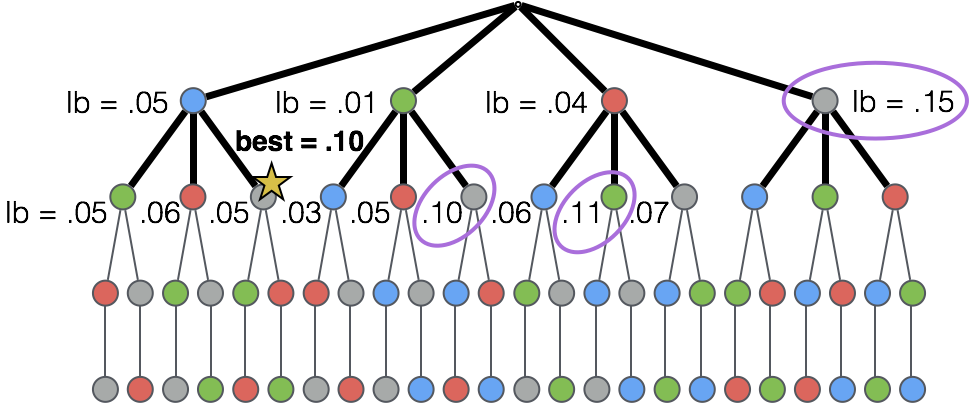
\includegraphics[width=0.5\textwidth]{figs/ela_branch-and-bound-tree.png}
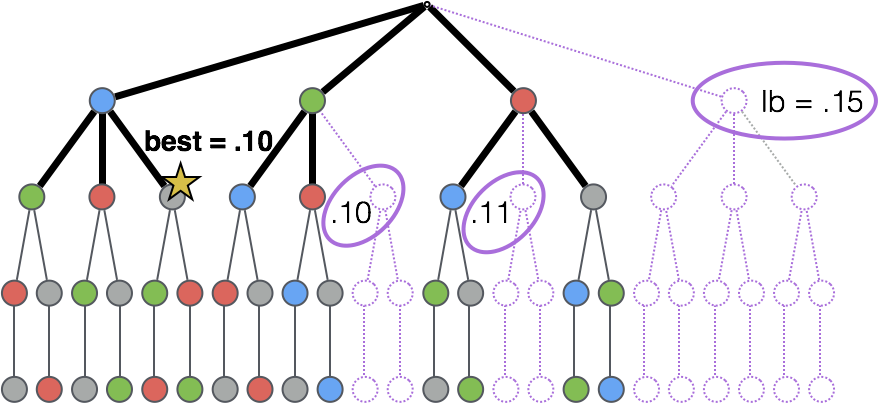
\includegraphics[width=0.5\textwidth]{figs/ela_branch-and-bound-tree-pruned.png}
\caption[Objective bound]{This tree shows the objective bound in action. Our best objective seen is the rule list (blue, gray) with an objective of $0.10$. Any rule lists with lower bound greater than this objective--(gray), (red, green), (green, gray) can be pruned and
\label{fig:objective-bound}}
\end{figure}

\subsubsection{Permutation Bound}

As defined above, every sample is captured by precisely one rule--any sample that is caught by rule A in the rule list AB cannot be caught by rule B. 
Now consider a permutation of the rule list AB: the rule list BA.
Any samples that are captured by either rule A or B but not both will be captured identically in both rule lists.
Samples that are captured by both rules will again be captured the same in both rule lists, though they may be predicted differently in the two rule lists.
Thus, regardless of the order in which the rules appear, rule lists AB and BA will capture exactly the same set data.
They will differ only in which rules capture which samples and therefore their accuracy may differ. 
We can use this knowledge to create a bound as follows.
If we know that the lower bound of AB is better than the lower bound of BA, we can eliminate from consideration all rule lists beginning with BA.
This is due to the fact that any corresponding rule list beginning with AB will capture exactly the same samples as the equivalent rule list beginning with BA but will have a better objective function.
We can eliminate all but one permutation of a given set of rules using this principle.

\subsubsection{Support Bound}
Due to our regularization term in calculating our objective function, adding a rule that does little to help our accuracy will actually be harmful to the overall objective score.
This allows us to place a bound intrinsic to the rule we're proposing adding.
We only consider adding rules that have capture enough data points correctly to overcome the regularization term.
Even though all rules have at least that support in the first case, as our rule lists get longer many rules do not capture enough points that haven't already been captured.

\subsubsection{Equivalent Points Bound}
This bound relies on the structure of our dataset.
In our dataset, we may encounter two data points that have the same features but different labels.
Thus, any rule that classifies one of the data points will also classify the other data point, but it is impossible to correctly predict both data points.
For a given class of equivalence points, therefore, we know that we will mispredict all of the points with a minority label.
We can thus update our lower bound to, by assuming that all uncaptured data will be correctly predicted only if it is not an equivalent point with a minority label.
This gives us much tighter lower bounds and in practice allows us to prune much more efficiently.

\subsection{Curiosity}
We have a number of different ways to explore the search space (see \ref{queue}).
Some of them, such as BFS prioritize exploration over exploitation.
Others, such as ordering by lower bound ensure that we are purely exploiting the best prefixes that we've seen.
We define a new metric, \textit{curiosity}, that is a function of both the lower bound and the number of samples captured.
This allows it to blend together both exploration and exploitation.

\subsection{Remaining Search Space}
Throughout this work, we will want to track how effective our bounds and other optimizations are.
One metric for tracking that will be seeing how quickly we reduce the remaining search space.
We start with a combinatorially large search space, but quickly prune it down.
The way we calculate the currently remaining search space is by looking at all of the leaves of the queue and seeing how much each leaf could potentially be expanded.
Due to our regularization term, we are able to bound the maximum length of a prefix as our best objective gets updated.

\section{Implementation}

This chapter lays out the design and implementation of the system used to generate optimal rule lists. 
We begin by describing each of the three main data structures used to run our algorithm--a prefix trie, a symmetry-aware map, and a queue. 
Then, we describe the overall execution of the key algorithm and provide a pseudocode version.

\subsection{Prefix Trie}
The prefix trie is a custom C++ class which is used as a cache to keep track of rule lists we have already evaluated. 
Each node in the trie contains the metadata associated with that corresponding rule list. 
This metadata includes bookkeeping information such as what child rule lists are feasible as well as information such as the lower bound and prediction for that rule list.
In addition to our BaseNode class, there are two different node types that we use in our algorithm.
Firstly, we implement a CuriousNode class that has an additional field that tracks the curiosity of a given prefix.
The curiosity metric is the one described in Chapter \ref{bounds}.
The curiosity is used to determine the order that prefixes on the queue are explored.
Secondly, we implement a CapturedNode class that extends on the CuriousNode by having an additional field keeping track of the captured vector for that prefix.
This allows us to speed up our incremental computations at the expense of using more memory per node (otherwise we have to recompute this vector every time we have a computation).

\subsection{Queue}
The various node types determine what type of search policy we use to explore the search space.
We use a STL C++ priority queue to hold all of the leaves of the trie that still need to be explored.
We implement a number of different scheduling schemes including BFS, DFS, and a priority queue.
The priority queue can be ordered by curiosity, the objective of a prefix, or the lower bound of a prefix.
We also have a stochastic exploration process that bypasses the use of a queue by walking down the trie, randomly choosing a child each time, until a leaf is chosen to be explored.
We find that ordering by curiosity will often, but not always, lead to a faster runtime than using BFS.

Since we do not have access to the container underlying the queue, we cannot randomly access elements in the queue, even if we have a pointer to the leaf node in the prefix trie.
Thus, we run into a problem where we may delete something in the prefix trie that is currently in the queue, but have no way to update the queue.
We deal with this by lazily deleting nodes from the prefix trie.
This means we mark the node as deleted in the trie, but don't actually delete the physical node until it has been popped off of the queue.
As Fig \ref{fig:queue_gc} shows, this leads to a situation where our logical queue is actually smaller than the physical queue.

\begin{figure}[t!]
\begin{center}
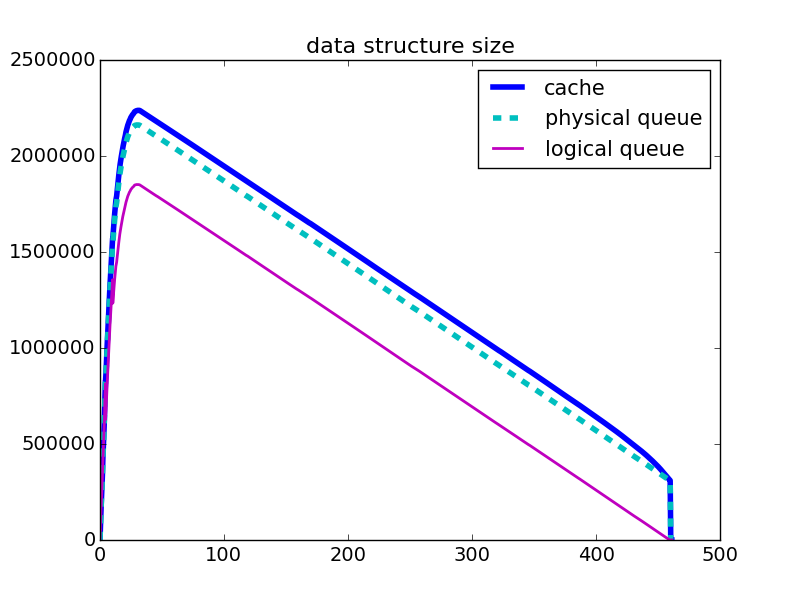
\includegraphics[width=0.65\textwidth]{figs/ela_compas-queue-cache-size-insertions.png}
\end{center}
\caption{Difference between logical cache and physical cache}
\label{fig:queue_gc}
\end{figure}

\subsection{Symmetry-aware map}
We implement the symmetry-aware map as an STL unordered\_map. 
We use this data structure to implement the permutation bound described in \ref{def:perm-bound}.
We have two different versions of the map with different keys that both allow permutations to be compared and pruned.
In both cases, the values contain the actual ordering of the rules that represents the current best prefix for that permutation.
In the first version, keys to the map are represented as the canonical order of rule lists: i.e. the lists 3-2-1 and 2-3-1 both map to 1-2-3.
The second version has keys that represent the captured data points.
Our earlier permutation bound was based off of the fact that different permutations capture the same data, so this type of key will again be equivalent for the rule lists 3-2-1 and 2-3-1.
Representing keys with captured vectors could potentially match more permutations, but requires more memory.
Since most data sets have a large amount of data, the keys representing the canonical ordering are usually more efficient.
In general, for long runs of our algorithm, the permutation map dominates our memory usage.

\subsection{Incremental execution}
Our program executes as follows. 
While there are still leaves of the trie to be explored, we use our scheduling policy to select the next rule list to evaluate.
Then, for every rule that is not already in this rule list, we calculate its lower bound, objective, and other metrics that would occur if the rule were added to the end of the rule list.
If the lower bound is greater than the minimum objective, meaning this new rule list could never be better than one we have already seen, we don't insert the new rule list into the tree or queue.
We next check if there is a better permutation of this rule list in the permutation map and discard the new rule list if it is not better than the rule list we already have in the permutation map.
If our new rule list is better, then we insert it into the permutation map, the tree, and the queue and update the minimum objective if necessary.

Every time we update the minimum objective, we garbage collect on the trie.
We do this by traversing from the root the all of the leaves, deleting any subtrees of nodes with a lower bound that is larger than the minimum objective.
In addition, if we encounter a node with no children, we prune upwards--deleting that node and recursively traversing the tree towards the root, deleting any childless nodes.
This garbage collection allows us to limit the memory usage of the trie, though garbage collection is not triggered too often.

\begin{algorithm}[t!]
  \caption{Branch-and-bound for learning rule lists}
\label{alg:branch-and-bound}
\begin{algorithmic}
\normalsize
\State $obj \gets 0$
\State $bestRL \gets NULL$
\State $T \gets initializeTree()$
\State $Q \gets queue(\,[T->root()\,])$
\State $P \gets map(\{\})$
\While {$Q$ not empty}
	\State $node \gets Q.pop()$
	\State $newObj \gets incremental(node, T, Q, P)$ \Comment{Evaluate all of node's children}
	\If {$newObj < obj$}
		\State $obj \gets newObj$
		\State $bestRL \gets node.getRuleList()$
		\State $T.garbageCollect()$
	\EndIf
\EndWhile


\end{algorithmic}
\end{algorithm}

\begin{algorithm}[t!]
  \caption{Incremental evaluation of a prefix}
\label{alg:incremental}
\begin{algorithmic}
\normalsize
\State \textbf{Input:} Node to be evaluated~n,
prefix tree~T,
queue~Q,
symmetry-aware map~P
\State \textbf{Output:} newObj~Best objective in the tree\\

\State 
\end{algorithmic}
\end{algorithm}


\section{Methodology}

\subsection{Improving Memory Usage of Symmetry-aware Map and Trie (Finding memory bottlenecks)}

Fixing the memory bloat of the symmetry aware map

$tt = ./bbcache -c 1 -n 100000 -p 1 -r 0.001 ../data/tdata\_R.out ../data/tdata\_R.label$
$tt_{reg} = ./bbcache -c 1 -n 100000 -p 1 -r 0.01 ../data/tdata\_R.out ../data/tdata\_R.label$

$bc = ./bbcache -c 1 -n 100000 -p 1 -r 0.001 ../data/bcancer.out ../data/bcancer.label$
$bc_{reg} = ./bbcache -c 1 -n 100000 -p 1 -r 0.01 ../data/bcancer.out ../data/bcancer.label$
$bc_{nodes} = ./bbcache -c 1 -n 1000000 -p 1 -r 0.001 ../data/bcancer.out ../data/bcancer.label$

$ad = ./bbcache -c 1 -n 100000 -p 1 -r 0.001 ../data/adult\_R.out ../data/adult\_R.label$
$ad_{reg} = ./bbcache -c 1 -n 100000 -p 1 -r 0.001 ../data/adult\_R.out ../data/adult\_R.label$
$ad_{nodes} = ./bbcache -c 1 -n 100000 -p 1 -r 0.001 ../data/adult\_R.out ../data/adult\_R.label$

\subsubsection{Keys as $std::set<size\_t>$, vals as $std::pair<std::vector<size\_t>, double>$}

\begin{center}
\begin{tabular} { |c|c|c|c|c|c|c| }
\hline
Name & \multicolumn{2}{c|}{Perm Map} & \multicolumn{2}{c|}{Tree} & time & accuracy \\
\hline
tt & 24928104 & 79.8\%  & 6317856 & 20.2\% & 17.601315 & 1.00000 \\

$tt_{reg}$ & 105849872 & 79.6\% & 27170304 & 20.4\% & 47.910126 & 1.00000 \\

bc &109281024 & 91.9\% & 9622752 & 8.1\% & 4.901384 & 0.98682 \\

$bc_{reg}$ & 197476840 & 74.9\% & 66004224 & 25.1\% & 438.309378 & 0.95168 \\

$bc_{nodes}$ & 1173870840 & 92.4\% & 96021408 & 7.6\% & 54.334499 & 0.98682 \\

ad & 36083664 & 79.0\% & 9614400 & 21.0\% & 4.485328 & 0.81048 \\

$ad_{reg}$ & 42119256 & 81.4\% & 9600768 & 18.6\% & 3.735894 & 0.81081 \\

$ad_{nodes}$ & 443942192 & 82.2\% & 96007296 & 17.8\% & 73.517540 & 0.81078 \\
\hline
\end{tabular}
\end{center}

\subsubsection{Keys as $std::vector<size\_t>$, vals as $std::pair<std::vector<size\_t>, double>$}

REPLACE NUMBERS

\begin{center}
\begin{tabular} { |c|c|c|c|c|c|c| }
\hline
Name & \multicolumn{2}{c|}{Perm Map} & \multicolumn{2}{c|}{Tree} & time & accuracy \\
\hline
tt & 24928104 & 79.8\%  & 6317856 & 20.2\% & 17.601315 & 1.00000 \\

$tt_{reg}$ & 105849872 & 79.6\% & 27170304 & 20.4\% & 47.910126 & 1.00000 \\

bc &109281024 & 91.9\% & 9622752 & 8.1\% & 4.901384 & 0.98682 \\

$bc_{reg}$ & 197476840 & 74.9\% & 66004224 & 25.1\% & 438.309378 & 0.95168 \\

$bc_{nodes}$ & 1173870840 & 92.4\% & 96021408 & 7.6\% & 54.334499 & 0.98682 \\

ad & 36083664 & 79.0\% & 9614400 & 21.0\% & 4.485328 & 0.81048 \\

$ad_{reg}$ & 42119256 & 81.4\% & 9600768 & 18.6\% & 3.735894 & 0.81081 \\

$ad_{nodes}$ & 443942192 & 82.2\% & 96007296 & 17.8\% & 73.517540 & 0.81078 \\
\hline
\end{tabular}
\end{center}

\subsubsection{Keys as $std::vector<unsigned short>$, vals as vals as $std::pair<std::vector<unsigned short>, double>$}

\begin{center}
\begin{tabular} { |c|c|c|c|c|c|c| }
\hline
Name & \multicolumn{2}{c|}{Perm Map} & \multicolumn{2}{c|}{Tree} & time & accuracy \\
\hline

tt & 7701812 & 57.1\%  & 5791368 & 42.9\% & 14.315976 & 1.00000 \\

$tt_{reg}$ & 36875368 & 59.4\% & 25160784 & 40.6\% & 42.896435 & 1.00000 \\

bc & 22464444 & 71.8\% & 8820856 & 28.2\% & 2.526981 & 0.98682 \\

$bc_{reg}$ & 77240290 & 56.1\% & 60503872 & 43.9\% & 404.327822 & 0.95168 \\

$bc_{nodes}$ & 230106908 & 72.3\% & 88019624 & 27.7\% & 27.476015 & 0.98682 \\

ad & 15292352 & 63.4\% & 8819800 & 36.6\% & 4.213340 & 0.81048 \\

$ad_{reg}$ & 16277360 & 64.9\% & 8811968 & 35.1\% & 3.525658 & 0.81081 \\

$ad_{nodes}$ & 160178964 & 64.5\% & 88161568 & 35.5\% & 47.643006 & 0.81078 \\
\hline
\end{tabular}
\end{center}

\subsubsection{Unordered map--Keys as $std::vector<unsigned short>$, vals as vals as $std::pair<std::vector<unsigned short>, double>$}

\begin{center}
\begin{tabular} { |c|c|c|c|c|c|c| }
\hline
Name & \multicolumn{2}{c|}{Perm Map} & \multicolumn{2}{c|}{Tree} & time & accuracy \\
\hline

tt & 7423740 & 56.2\%  & 5791368 & 43.8\% & 13.609930 & 1.00000 \\

$tt_{reg}$ & 35661696 & 58.6\% & 25160784 & 41.4\% & 42.945947 & 1.00000 \\

bc & 21698948 & 71.1\% & 8820856 & 28.9\% & 2.138304 & 0.98682 \\

$bc_{reg}$ & 72839418 & 54.6\% & 60503872 & 45.4\% & 359.959682 & 0.95168 \\

$bc_{nodes}$ & 227288484 & 72.1\% & 88019624 & 27.9\% & 21.061545 & 0.98682 \\

ad & 14746584 & 62.6\% & 8819800 & 37.4\% & 3.402276 & 0.81048 \\

$ad_{reg}$ & 15641304 & 64.0\% & 8811968 & 36.0\% & 3.106825 & 0.81081 \\

$ad_{nodes}$ & 159236876 & 64.4\% & 88161568 & 35.6\% & 43.151872 & 0.81078 \\
\hline
\end{tabular}
\end{center}

\subsubsection{Unordered map--Keys as $unsigned short *$, vals as vals as $std::pair<std::vector<unsigned short>, double>$}

\begin{center}
\begin{tabular} { |c|c|c|c|c|c|c| }
\hline
Name & \multicolumn{2}{c|}{Perm Map} & \multicolumn{2}{c|}{Tree} & time & accuracy \\
\hline

tt & 5539628 & 48.9\%  & 5791368 & 51.1\% & 16.437973 & 1.00000 \\

$tt_{reg}$ & 28019470 & 52.7\% & 25160784 & 47.3\% & 40.594612 & 1.00000 \\

bc & 16164866 & 64.7\% & 8820856 & 35.3\% & 2.175347 & 0.98682 \\

$bc_{reg}$ & 56388394 & 48.2\% & 60503872 & 51.8\% & 371.937364 & 0.95168 \\

$bc_{nodes}$ & 168402474 & 65.7\% & 88019624 & 34.3\% & 19.322026 & 0.98682 \\

ad & 12403876 & 58.4\% & 8819800 & 41.6\% & 3.230369 & 0.81048 \\

$ad_{reg}$ &12987184 & 59.6\% & 8811968 & 40.4\% & 2.809433 & 0.81081 \\

$ad_{nodes}$ & 131981438 & 60.0\% & 88161568 & 40.0\% & 43.882791 & 0.81078 \\
\hline
\end{tabular}
\end{center}

\subsubsection{Above (3.1.5) and reordering tree nodes}

\begin{center}
\begin{tabular} { |c|c|c|c|c|c|c| }
\hline
Name & \multicolumn{2}{c|}{Perm Map} & \multicolumn{2}{c|}{Tree} & time & accuracy \\
\hline

tt & 5539620 & 51.3\%  & 5264880 & 48.7\% & 15.787402 & 1.00000 \\

$tt_{reg}$ & 28019462 & 55.1\% & 22873440 & 44.9\% & 35.468984 & 1.00000 \\

bc & 16164858 & 66.8\% & 8018960 & 33.2\% & 1.933180 & 0.98682 \\

$bc_{reg}$ & 56388386 & 50.6\% & 55003520 & 49.4\% & 345.475240 & 0.95168 \\

$bc_{nodes}$ & 168402466 & 67.8\% & 80017840 & 32.2\% & 19.360888 & 0.98682 \\

ad & 12403868 & 60.7\% & 8018000 & 39.3\% & 3.121322 & 0.81048 \\

$ad_{reg}$ & 12987176 & 61.8\% & 8010880 & 38.2\% & 2.703331 & 0.81081 \\

$ad_{nodes}$ & 131981430 & 62.2\% & 80146880 & 37.8\% & 37.732368 & 0.81078 \\
\hline
\end{tabular}
\end{center}

\subsubsection{Unordered map--Keys as $unsigned short *$, vals as vals as $std::pair<double, unsigned char*>$}

\begin{center}
\begin{tabular} { |c|c|c|c|c|c|c| }
\hline
Name & \multicolumn{2}{c|}{Perm Map} & \multicolumn{2}{c|}{Tree} & time & accuracy \\
\hline

tt & 3655508 & 41.0\%  & 5264880 & 59.0\% & 13.046520 & 1.00000 \\

$tt_{reg}$ & 20377236 & 47.1\% & 22873440 & 52.9\% & 52.318813 & 1.00000 \\

bc & 10630776 & 57.0\% & 8018960 & 43.0\% & 2.184780 & 0.98682 \\

$bc_{reg}$ & 39937362 & 42.1\% & 55003520 & 57.9\% & 399.382231 & 0.95168 \\

$bc_{nodes}$ & 109516456 & 57.8\% & 80017840 & 42.2\% & 21.461987 & 0.98682 \\

ad & 10113288 & 55.8\% & 8019680 & 44.2\% & 3.390032 & 0.81048 \\

$ad_{reg}$ &10333056 & 56.3\% & 8010880 & 43.7\% & 3.096620 & 0.81081 \\

$ad_{nodes}$ & 104855160 & 56.7\% & 80150800 & 43.3\% & 43.222397 & 0.81078 \\
\hline
\end{tabular}
\end{center}

\subsubsection{Ordered map--Keys as $std::vector<bool>$, values as $std::vector<unsigned short>, double$}

\begin{center}
\begin{tabular} { |c|c|c|c|c|c|c| }
\hline
Name & \multicolumn{2}{c|}{Perm Map} & \multicolumn{2}{c|}{Tree} & time & accuracy \\
\hline

tt & 11413638 & 68.4\%  & 5274016 & 31.6\% & 14.426219 & 1.00000 \\

$tt_{reg}$ & 55946962 & 69.3\% & 24777016 & 30.7\% & 42.086578 & 1.00000 \\

bc & 14602388 & 62.3\% & 8822616 & 37.7\% & 266.859001 & 0.98829 \\

$bc_{reg}$ & 125912468 & 68.7\% & 57428448 & 31.3\% & 295.119223 & 0.95168 \\

$bc_{nodes}$ & 126686680 & 58.9\% & 88285032 & 41.1\% & 4430.965258 & 0.98829 \\

ad & 267807290 & 96.8\% & 8804224 & 3.2\% & 71.885551 & 0.81078 \\

$ad_{reg}$ & 356845610 & 97.6\% & 8816632 & 2.4\% & 53.843208 & 0.81081 \\

$ad_{nodes}$ & 1018150922 & 97.4 \% & 88000704 & 2.6 \% & 7005.960590 &  0.81078\\
\hline
\end{tabular}
\end{center}

\subsubsection{Ordered map--Keys as $VECTOR$, values as $std::vector<unsigned short>, double$}

\begin{center}
\begin{tabular} { |c|c|c|c|c|c|c| }
\hline
Name & \multicolumn{2}{c|}{Perm Map} & \multicolumn{2}{c|}{Tree} & time & accuracy \\
\hline

tt & 5791368 & 61.3\%  & 3658580 & 38.7\% & 10.644521 & 1.00000 \\

$tt_{reg}$ & 25160784 & 55.2\% & 20380308 & 44.8\% & 33.295206 & 1.00000 \\

bc & 10641520 & 54.7\% &8820856 & 45.3\% & 0.914455 & 0.98682 \\

$bc_{reg}$ & 60503872 & 60.2\% & 39948106 & 39.8\% & 309.314620 & 0.95168 \\

$bc_{nodes}$ & 109527200 & 55.4\% & 88019624 & 44.6\% & 11.085341 & 0.98682 \\

ad & 10115616 & 53.4\% & 8821648 & 46.6\% & 3.169979 & 0.81048 \\

$ad_{reg}$ & 10335384 & 54.0\% & 8811968 & 46.0\% & 2.126727 & 0.81081 \\

$ad_{nodes}$ & 104857488 & 54.3 \% & 88165880 & 45.7 \% & 38.948489 &  0.81078\\
\hline
\end{tabular}
\end{center}

\subsection{Parallelizing Execution}

file:///Users/nlarusstone/Downloads/eur-few-cs-95-04.pdf

Begin by trying to run multiple threads on a stochastic selection algorithm.

Initially coarse locking on the entire tree--share both the tree and permutation map in memory
No--actually no permutation map, no locking, no garbage collection
	Threadpool to run the evaluate children (because that's where the majority of work is done)
	Locking is causing a lot of contention and is difficult to get reliable results

Can't parallelize the for loop inside evaluate children
	Without synchronization, turns out that the insertion of a child into its parent's children\_ map can lead to a null access if the underlying tree rebalances
	Synchronization causes too much contention on that lock, so will want our threads to be working on different parts of the tree instead of trying to speed up calculations for a single prefix

Partition tree from top
	Each worker starts with (nrules/num\_threads) rules in its tree and then it can add whatever rules it would like after that.

\subsection{How much does each bound help? (Finding time bottlenecks)}

\subsection{Investigating similarity of prefixes}

\subsection{Cached bit vector node}

\subsection{Exploration of nearly-optimal rule lists and comparisons to other algorithms}

\subsection{Inheritance vs Templating}


With pure templates:
Executable size: 253732
-c 1 -n 100000 -p 1 -r 0.001 ../data/tdata\_R.out ../data/tdata\_R.label: 11.191856
-c 1 -n 100000 -p 1 -r 0.001 ../data/bcancer.out ../data/bcancer.label: 1.188271
-c 1 -n 100000 -p 1 -r 0.001 ../data/adult\_R.out ../data/adult\_R.label: 2.906099
-c 1 -n 100000 -p 1 -r 0.001 ../data/compas.out ../data/compas.label: 4.038996

$10^7$ nodes
9.822864 8.850554 8.943174
77.118279 68.101442 63.307958
416.428278 399.025332 404.614529
427.698726 427.517602 410.294034

$10^7$ (Commented out logger)
8.705810 (8.829541)
58.472542 (53.311810)
372.558429 (249.713447)
398.003311 (103.392936)

Inherited queue:
Executable size: 249484
9.461418
1.324893
3.158447
4.354028

Inherited queue + pmap:
Executable size: 209876
9.192366
1.068136
3.257429
4.484909

$10^7$ nodes
8.968495 9.562288 10.391837
70.315091 66.474482 70.032368
395.544781 388.303023 402.497634
448.220752 508.278413 453.807489

Pure Inheritance:
Executable size: 171288
$10^7$ nodes
13.433584 12.546750
64.704144 60.598935
200.708991 187.573605
127.951469 111.120107

Logger with return statements:
9.263342
60.493697
203.016282
110.914362

With NullLogger (no-op virtual functions):
8.918576
55.236019
185.749401
105.225227

With Logger as an inherited class:
9.039654
56.637848
190.003558
107.623293


\subsection{Applications: COMPAS, Medical, Credit Scoring, ASC, Neural Nets}

COMPAS:
%http://www.crj.org/page/-/publications/rejoinder7.11.pdf

Credit Scoring:
%Have to provide a reason for why an application is rejected

NNs:
%http://citeseerx.ist.psu.edu/viewdoc/download?doi=10.1.1.12.6011&rep=rep1&type=pdf
%https://www.biostat.wisc.edu/~craven/papers/thesis.pdf

\printbibliography

\end{document}